\documentclass{article}
\usepackage[paperwidth=8.8cm,paperheight=10cm,margin=1mm]{geometry}
\usepackage{tikz}
\usepackage{graphicx}
\pagestyle{empty}

\begin{document}
\noindent
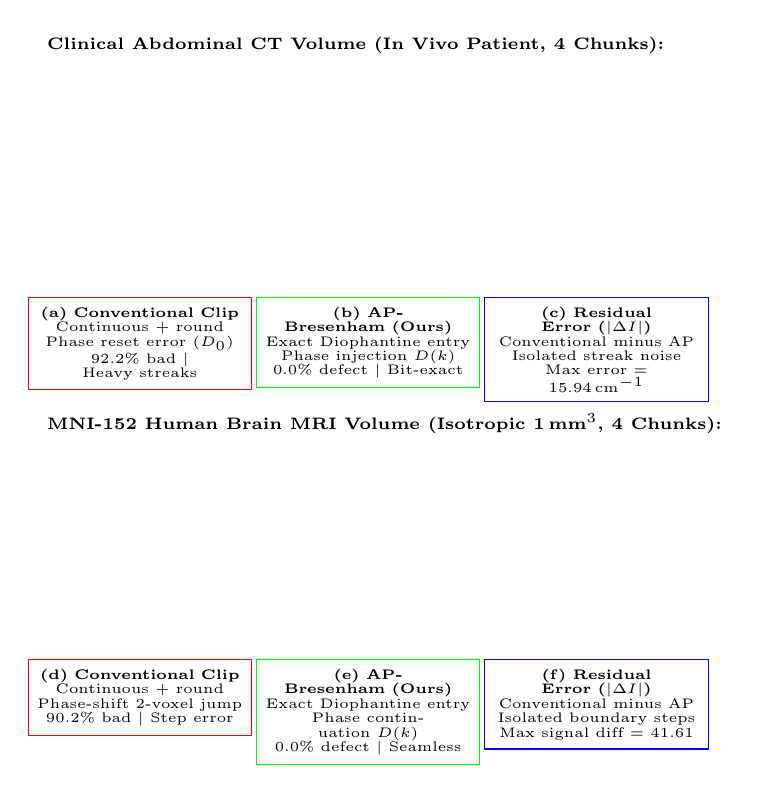
\begin{tikzpicture}[font=\sffamily]

% Row 1
\node[anchor=west, font=\fontsize{6.0pt}{7.0pt}\bfseries\selectfont] at (0.2, 9.4) 
    {Clinical Abdominal CT Volume (In Vivo Patient, 4 Chunks):};

\node[anchor=north, align=center, text width=2.6cm, font=\fontsize{4.2pt}{5.2pt}\selectfont, draw=red] at (1.50, 6.2) {
    \textbf{(a) Conventional Clip}\\
    Continuous + round\\
    Phase reset error ($D_0$)\\
    92.2\% bad $\mid$ Heavy streaks
};

\node[anchor=north, align=center, text width=2.6cm, font=\fontsize{4.2pt}{5.2pt}\selectfont, draw=green] at (4.40, 6.2) {
    \textbf{(b) AP-Bresenham (Ours)}\\
    Exact Diophantine entry\\
    Phase injection $D(k)$\\
    0.0\% defect $\mid$ Bit-exact
};

\node[anchor=north, align=center, text width=2.6cm, font=\fontsize{4.2pt}{5.2pt}\selectfont, draw=blue] at (7.30, 6.2) {
    \textbf{(c) Residual Error ($|\Delta I|$)}\\
    Conventional minus AP\\
    Isolated streak noise\\
    Max error = 15.94\,cm$^{-1}$
};

% Row 2
\node[anchor=west, font=\fontsize{6.0pt}{7.0pt}\bfseries\selectfont] at (0.2, 4.6) 
    {MNI-152 Human Brain MRI Volume (Isotropic 1\,mm$^3$, 4 Chunks):};

\node[anchor=north, align=center, text width=2.6cm, font=\fontsize{4.2pt}{5.2pt}\selectfont, draw=red] at (1.50, 1.6) {
    \textbf{(d) Conventional Clip}\\
    Continuous + round\\
    Phase-shift 2-voxel jump\\
    90.2\% bad $\mid$ Step error
};

\node[anchor=north, align=center, text width=2.6cm, font=\fontsize{4.2pt}{5.2pt}\selectfont, draw=green] at (4.40, 1.6) {
    \textbf{(e) AP-Bresenham (Ours)}\\
    Exact Diophantine entry\\
    Phase continuation $D(k)$\\
    0.0\% defect $\mid$ Seamless
};

\node[anchor=north, align=center, text width=2.6cm, font=\fontsize{4.2pt}{5.2pt}\selectfont, draw=blue] at (7.30, 1.6) {
    \textbf{(f) Residual Error ($|\Delta I|$)}\\
    Conventional minus AP\\
    Isolated boundary steps\\
    Max signal diff = 41.61
};

\end{tikzpicture}
\end{document}

